\chapter{Phenomenological modeling of our HETGs data}
\section{Introduction to Our Observation}
During 2018 August 10-14, SS 433 was observed using the High Energy Transmission Grating Spectrometer System (HETGS) on the Chandra X-ray Observatory. The full observing plan consisted of two parts. The first part is a 20 ksec observation, which was taken 3 days before the accretor was completely blocked by the donor (an eclipse) (See Figure~\ref{video_short} for the geometry). The orbital phase of the starting of the observation was 0.802. The second part was a 96 ksec long observation, which started right at the middle of the eclipse (See Figure~\ref{video_long1} and \ref{video_long2} for the geometry). The purpose of this observation was to use the eclipse of the accretor by the donor to map out the spatial variation of the jet's properties such as temperature, density ionization state, bulk jet-speed, composition, etc. We hoped to achieve our objective by comparing and analyzing spectra from two observations. In this chapter, we describe spectral fitting with phenomenological models, using line-grouping method and the blind search method. \par 


\begin{figure}
    \centering
    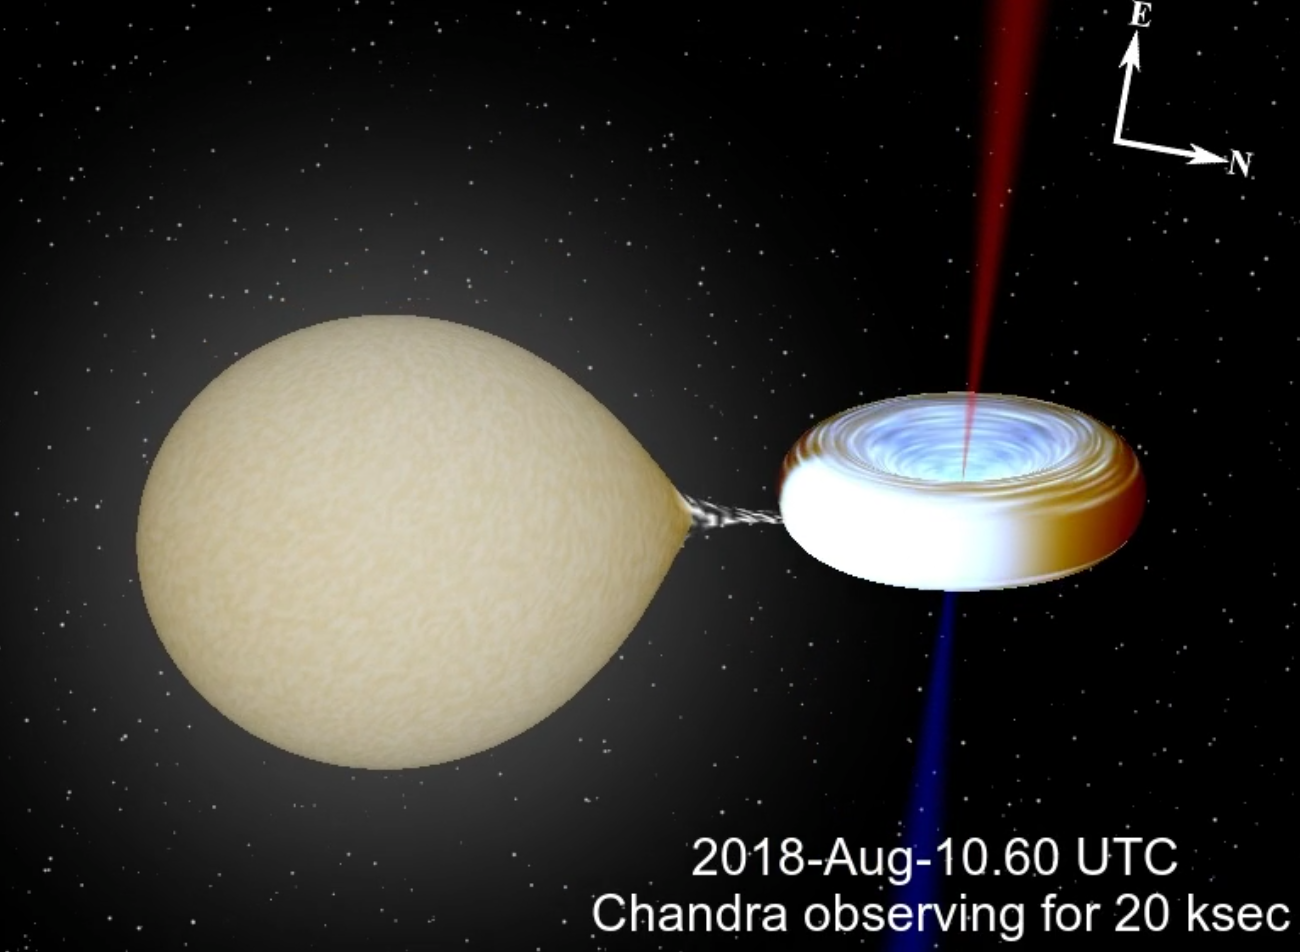
\includegraphics[scale = 0.2]{Chapters/Figures/video_short.png}
    \caption{The geometry of the starting time of the 20 ksec observation.}
    \label{video_short}
\end{figure}

\begin{figure}[h!]
    \centering
    \begin{subfigure}[t]{.4\textwidth}
        \centering
        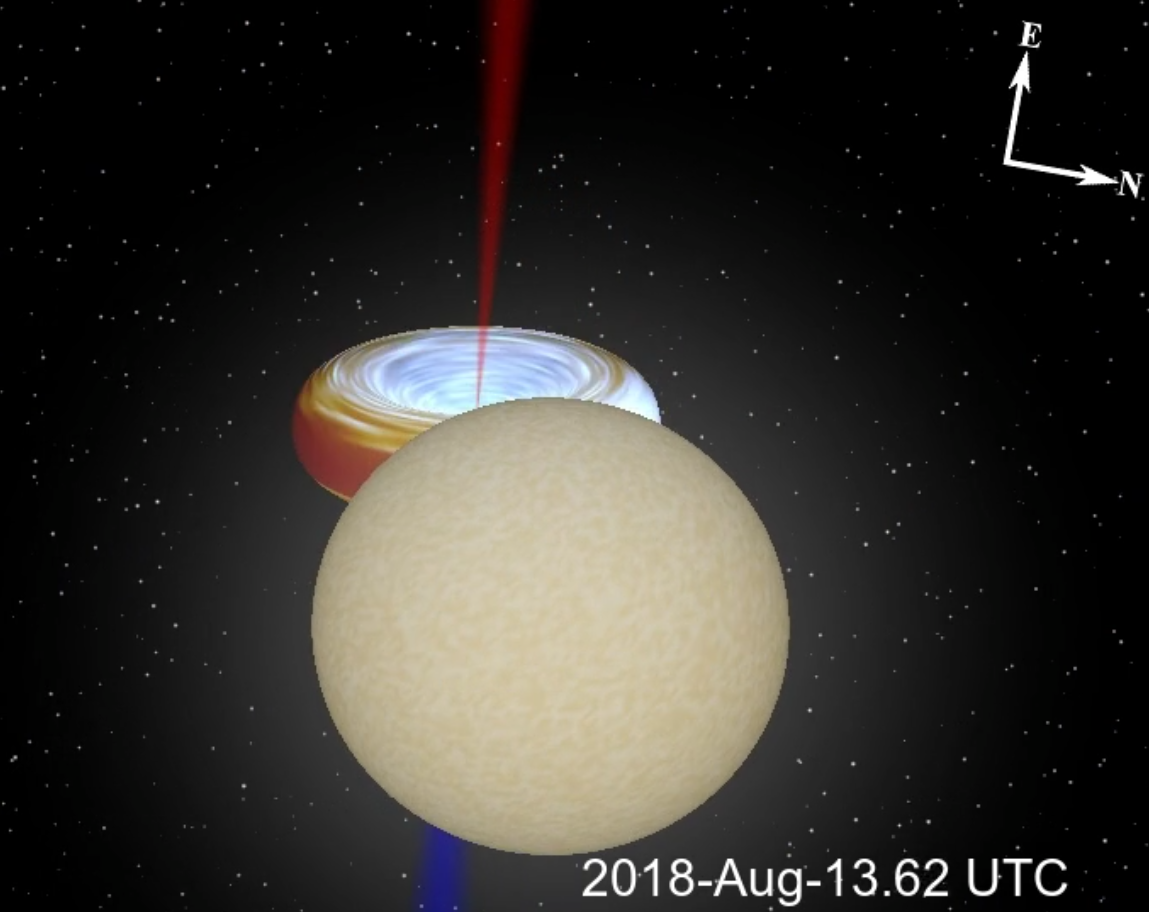
\includegraphics[width=0.94\linewidth]{Chapters/Figures/video_long.png}
        \caption{The geometry of the starting point of the 96 ksec observation.}
        \label{video_long1}
    \end{subfigure}%
    \hspace*{4em}
    \begin{subfigure}[t]{.4\textwidth}
        \centering
        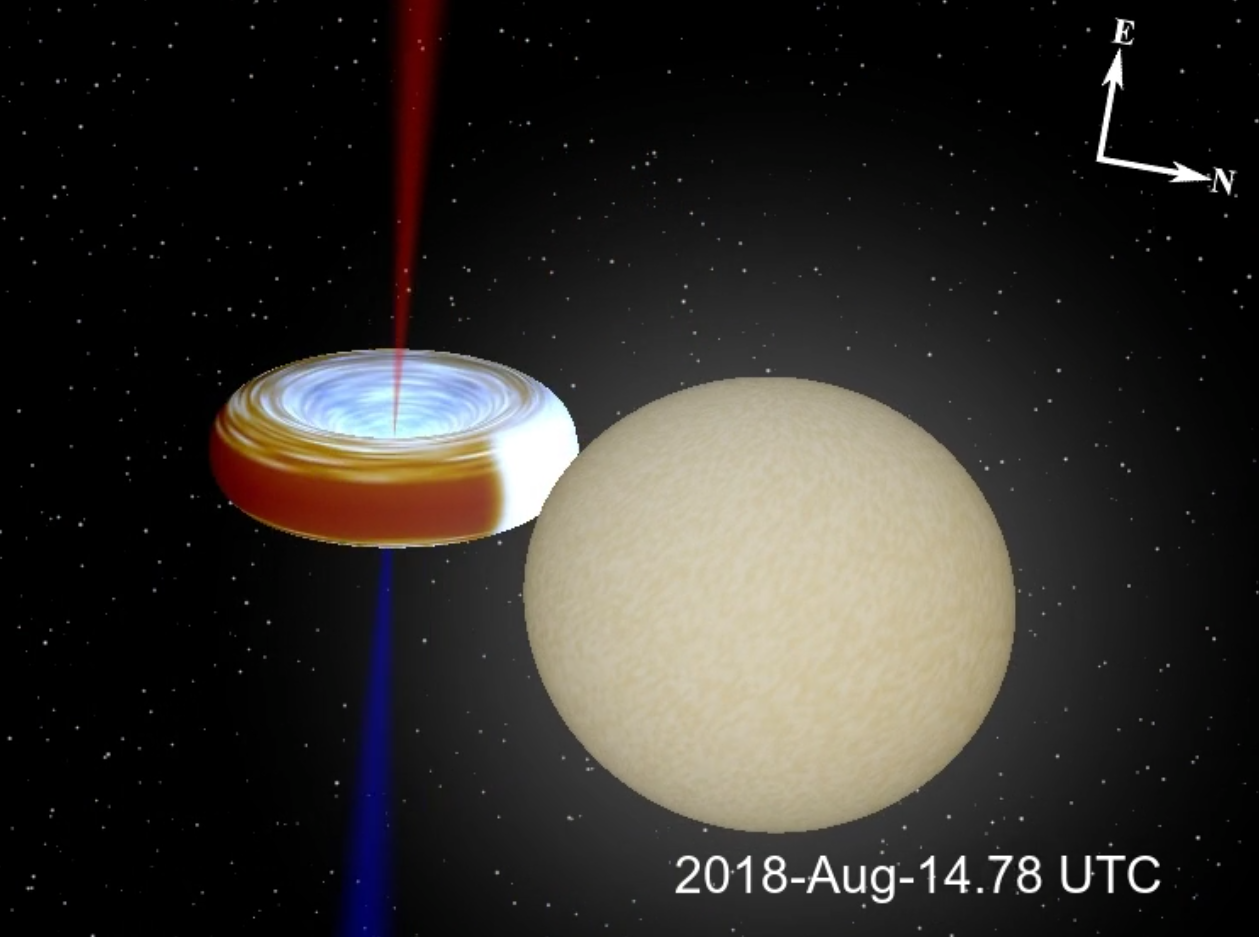
\includegraphics[width=\linewidth]{Chapters/Figures/video_long2.png}
        \caption{The geometry of the ending point of the 96 ksec observation.}
        \label{video_long2}
    \end{subfigure}
    \label{video_long}
\end{figure}




\section{The 20 ksec Observation on August 10, 2018}
\subsection{Method}
The emission lines on the spectra usually tell the most about the properties of the jets. The summary plots produced by TGCAT \citep{Huenemoerder2011} give a general idea of where the emission lines are (see Figure~\ref{summaryplot_el}). Previous papers \citep{Marshall2002, Marshall2013, Lopez2006} show the corresponding rest wavelengths of normal emission lines from those heavy elements. There are also other ways to access the accurate emission line wavelengths database. The X-Ray Data Booklet \citep{thompson2001} shows a complete energies of X-ray emission lines. The corresponding wavelengths can be found by 
\begin{equation}
    E = hc/\lambda.
\end{equation}


\begin{figure}
    \centering
    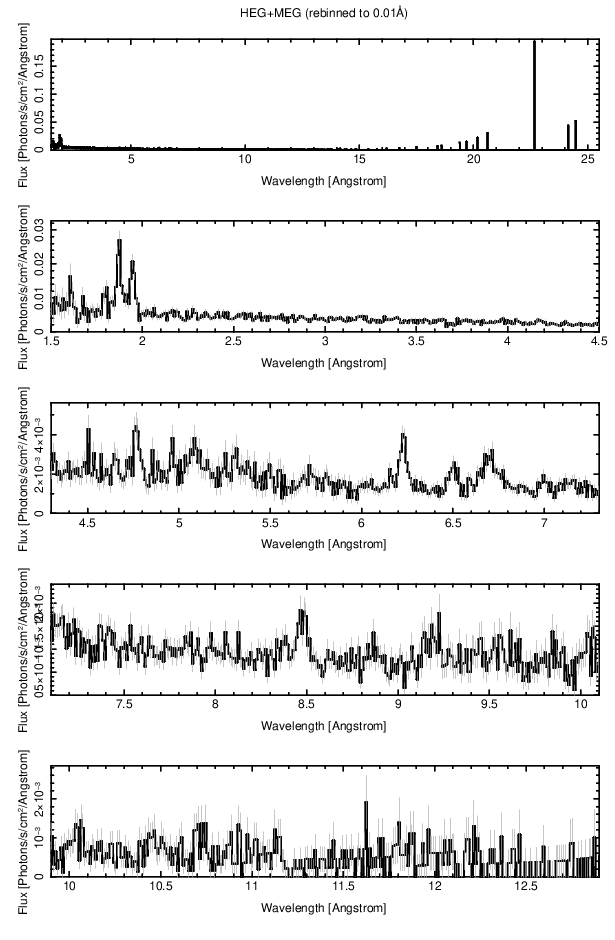
\includegraphics[width = 0.7\linewidth]{Chapters/Figures/summaryplot_el.png}
    \caption{A summary plot of 2018-08-10 Chandra observation produced by TGCAT \citep{Huenemoerder2011}. The plot shows the line fluxes over wavelength. }
    \label{summaryplot_el}
\end{figure}

Phenomenological models (models that describe the observed data, but are not directly derived from any physically motivated theory) are built to fit the continuum spectrum and the emission lines so that the line fluxes as well as the continuum's properties can be measured and studied. \par 
%This model determines the best redshift value of a jet by fitting all observed emission lines from one jet based on its rest wavelength and the redshift of the jet. 

After generating the PHA file and the corresponding ARF and RMF files, using a script written in ISIS to fit the group-line model to the spectrum. The script initially loads the APED so that theoretical wavelengths, radiative transition rates, and electron collisional excitation rate coefficients for most known X-ray transitions can be accessed. \par 
To simplify the fitting process, we start by fitting a few line profiles to a small part of the spectrum. Therefore, it is important to initially ignore all other spectra and all bins outside the region of interest. \par 
Usually one does not want to use the full resolution of a spectrum, either because the channels oversample the spectral resolution or because the signal-to-noise ratio for each bin is low. It is effective to assign the values to groups, to create a smaller set of discrete ranges. For our data, we grouped every 4 PHA channels in the MEG (or the HEG) together. Then we ignored a certain range of HEG and MEG data due to lack of good calibration data in these range. After excluding these energies, we used 1.25 - 10 \AA\ range of HEG data and 2.5 - 13 \AA\ range of MEG data. \par 


Since we know the orbital period and the precession period of the binary, we computed the predicted redshift values for both red and blue jets with a C program based on the kinematic model \citep{Margon1979}. Given the MJD (Modified Julian Date: number of days after midnight on November 17, 1858) of the observation, the program computes the corresponding predicted redshifts for both Western and Eastern jets at certain times. For the precession phase of our 20 ksec observation, the predicted blue- and red-shifts were 0.009234 and 0.06791 for the Western and Eastern jet, respectively. \par

\subsubsection{Line-grouped Model}
One of the models used here is called the line-grouped model. Precise redshift for these emission line profiles were determined by fitting lines from the same jet together with several Gaussian components of known rest wavelength values taken from Astrophysical Plasma Emission Database (APED) \citep{smith2001}.\par
We define a fit function which is a combination of multiplicative models and additive models. \textbf{wabs} is a multiplicative model that describes photoelectric absorption due to neutral gas between us and SS 433 \citep{Arnaud1999}. It modifies the observed spectrum so that the spectrum has a proper continuum. In the additive model, there are two main components. The first one is a power law, fitting the continuum spectrum 
\begin{equation}
     N(E) = KE^{-\alpha},
     \label{powerlaweq}
\end{equation}
where $K$ is photons/keV/cm$^2$/s at 1 keV and $\alpha$ is the photon index. The second one is the sum of many Gaussian distributions
\begin{equation}
     N(E) = K\dfrac{1}{\sigma \sqrt{2\pi}}\mathrm{exp}(\dfrac{-(E-E_l)^2}{2\sigma^2}, 
\end{equation}
where $K$ is the total photons/cm$^{-2}$/s in the line, $E_l$ is line energy in keV and $\sigma$ is line width in keV. Each emission line profile is modeled using one Gaussian.\par 

After defining the fitting function, we set the parameter values. The parameters include the starting best-guess values of two redshifts (one for each jet), two error terms for the redshifts, the rest wavelengths of all the elements, Gaussian widths and Gaussian areas. Since there are many parameters to fit, we give a physically plausible search range for each of the parameter, thereby speeding up the convergence of the fitting. \par 

Cash statistic was applied to find the best model fit to the data, which means the least model deviation from the data. Lines were fitted to the MEG and HEG data separately in their own wavelength ranges. Precise redshifts of both jets for these profiles were determined by fitting the emission lines of known rest wavelength values.\par


\subsubsection{Blind Fitting Method}

To determine the wavelengths and fluxes of the observed emission lines and their errors, we used a blind fitting method to fit the spectra. In this method, Voigt function, similar to Gaussian, is used to fit the emission lines. The Voigt profile is the convolution of the natural resonance of an emitted line with the Maxwellian speed distribution \citep{Houck2000}. The natural resonance profile is a Lorentzian with full-width at half maximum, $\Gamma/4\pi$. The Maxwellian speed distribution is a Gaussian with velocity width $v_o = \left(\dfrac{2kT}{m}\right)^{1/2}$, where $m$ is the ion mass and $T$ is the temperature. Unlike the previous fitting method, this fitting model does not depend on redshift. By indicating the center of an emission line, the model is fit to the spectra.

\subsection{Results}

The spectra are shown in Figure~\ref{shorthegpheno} - Figure~\ref{shortmegpheno}. Similar to previous observations, typical emission lines of irons, nickel, sulfur, and silicon and a significant continuum are prevalent. Emission lines from the Western and Eastern jets are prominent enough to find the  accurate measurement of redshifts for both jets. \par

\begin{figure}[h!]
    \centering
    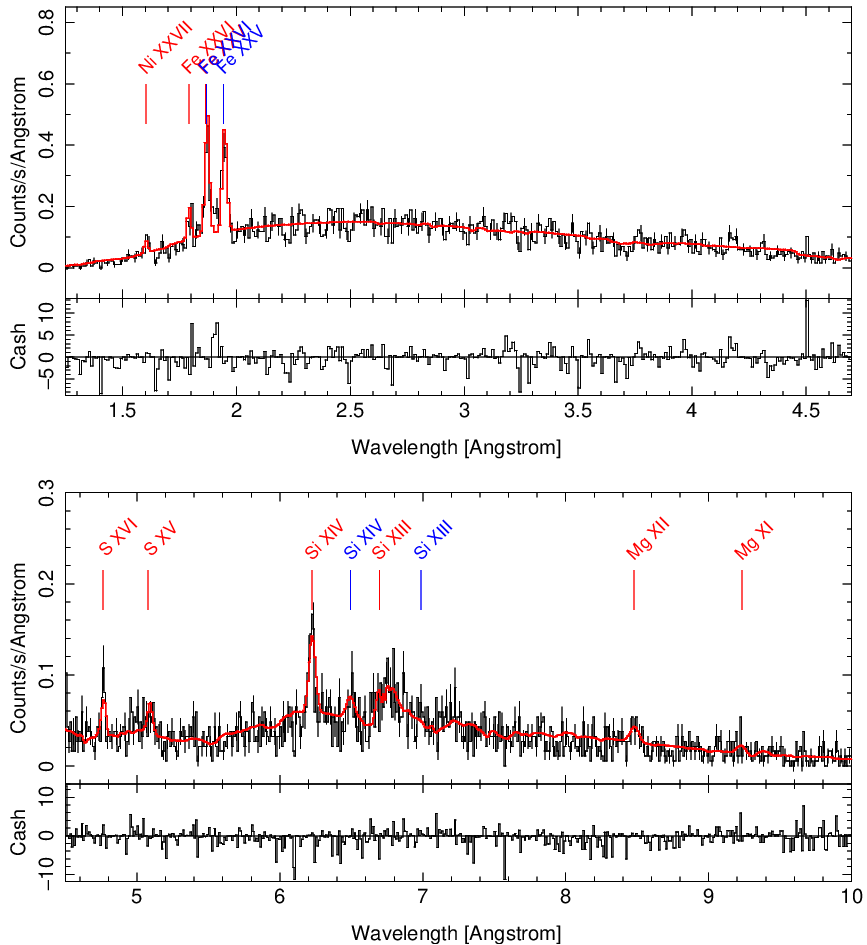
\includegraphics[width = \linewidth]{Chapters/Figures/short_pheno_heg.png}
    \caption{The 20 ksec X-ray spectrum of SS 433 observed with the Chandra HETGS on 2018-08-10. This set of figures show the spectrum from the HEG data. The Bremsstrahlung radiation likely creates the continuum. Red line: phenomenological model fit to the spectrum from 1.25\AA -  10\AA. Line identifications are labeled where there are features in the spectrum and confirmed by the model. The red characters label the emission lines from the Western jet while the blue ones from the Eastern jet. The Cash statistic residuals are shown at the bottom of each spectrum. }
    \label{shorthegpheno}
\end{figure}



\begin{figure}[h!]
    \centering
    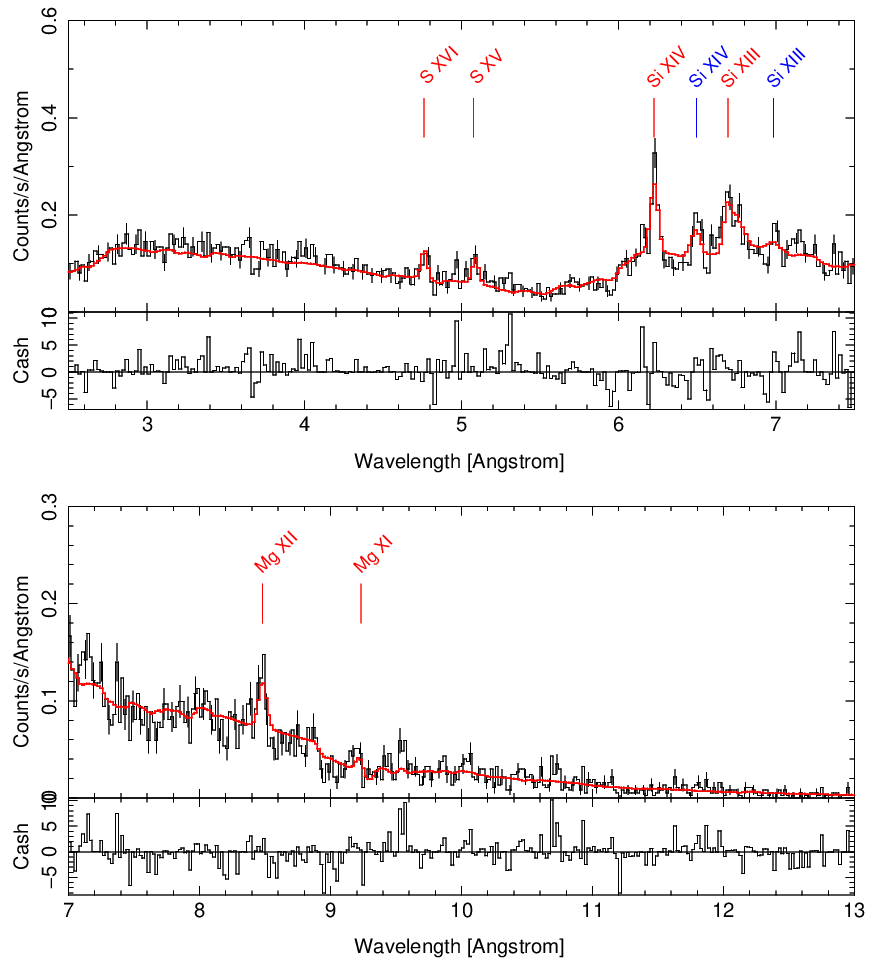
\includegraphics[width = \linewidth]{Chapters/Figures/short_pheno_meg.png}
    \caption{Same as Figure~\ref{shorthegpheno} but showing the X-ray spectrum of SS 433 from the MEG data. Red line: phenomenological model fit to the spectrum from 2.5\AA -  13\AA.}
    \label{shortmegpheno}
\end{figure}

\newpage
\newpage
\newpage
The line fluxes are shown in Table~\ref{tab:shortlinefluxes_west} - \ref{tab:shortlinefluxes_east}.  $z$ denotes the redshift. There are more detectable lines from the Western jet than the Eastern jet as predicted since our observation was taken when the Western jet is approaching while the Eastern jet is receding. The Eastern jet will be somewhat fainter than the Western jet, when there was a large difference in the Eastern and Western Doppler shifts. \par 




\begin{deluxetable}{lccccr}
\tablecolumns{5}
\tablewidth{0pc}
\tabletypesize{\small}
\tablecaption{SS 433 Western Jet Line Diagnostics Using Voigt profiles for the 20 ksec Observation
\label{tab:shortlinefluxes_west}\tablenotemark{a} }
\tablehead{\colhead{Identification}& \colhead{$\lambda_{\rm rest}$} & \colhead{$\lambda_{\rm obs}$} & \colhead{$z$}
    & \colhead{Line Flux}  & \colhead{$\sigma$} \\
  \colhead{}& \colhead{(\AA)} & \colhead{(\AA)} & \colhead{}
    & \colhead{($10^{-6}$ ph \mathrm{cm$^{-2}$ s$^{-1}$})} & \colhead{\AA} }
\startdata
Ni{\sc xxvii}&	1.592&	1.608$\pm$	0.003&	0.0102$\pm$0.0018&	221.5$\pm$59.1&	0.0055\\
Fe{\sc xxvi}&	1.78&	1.798$\pm$	0.003&	0.0103$\pm$0.0014&	187.6$\pm$37.7&	0.0062\\
Fe{\sc xxv}&	1.855&	1.875$\pm$	0.001&	0.0107$\pm$0.0006&	459.1$\pm$49.5&	0.0064\\
S{\sc xvi}&	4.73&	4.767$\pm$	0.021&	0.0078$\pm$0.0044&	50$\pm$2&	0.0164\\
S{\sc xv}&	5.055&	5.084$\pm$	0.011&	0.0058$\pm$0.0021&	119.7$\pm$31&	0.0175\\
Si{\sc xiv}&	6.182&	6.227$\pm$	0.002&	0.0073$\pm$0.0003&	150$\pm$5.1&	0.0214\\
Si{\sc xiii}r&	6.648&	6.675$\pm$	0.005&	0.0041$\pm$0.0007&	59.9$\pm$10.4&	0.023\\
Si{\sc xiii}i&	6.687&	6.71$\pm$	0.004&	0.0035$\pm$0.0006&	78.3$\pm$12.1&	0.0232\\
Si{\sc xiii}f&	6.74&	6.761$\pm$	0.002&	0.0031$\pm$0.0003&	50.2$\pm$2&	0.0234\\
Mg{\sc xii}&	8.421&	8.472$\pm$	0.005&	0.0061$\pm$0.0005&	92.2$\pm$11.4&	0.0292\\
Mg{\sc xi}&	9.169&	9.188$\pm$	0.012&	0.002$\pm$0.0013&	86.2$\pm$15&	0.0318\\
\enddata
\tablenotetext{a}{All uncertainties refer to statistical 90\% confidence limits}
\end{deluxetable}


\begin{deluxetable}{rcccr}
\tablecolumns{5}
\tablewidth{0pc}
\tabletypesize{\small}
\tablecaption{SS 433 Eastern Jet Line Diagnostics Using  Voigt profiles for the 20 ksec Observation\tablenotemark{a}
\label{tab:shortlinefluxes_east} }
\tablehead{ \colhead{Identification}& \colhead{$\lambda_{\rm rest}$} & \colhead{$\lambda_{\rm obs}$} & \colhead{$z$}
    & \colhead{Line Flux}  & \colhead{$\sigma$} \\
   \colhead{} &\colhead{(\AA)} & \colhead{(\AA)} & \colhead{}
    & \colhead{($10^{-6}$ ph cm$^{-2}$ s$^{-1}$)} & \colhead{\AA}}
\startdata
Fe {\sc xxvi}& 1.78&	1.864 $\pm$ 0.002&	0.0471 $\pm$ 0.0011&	266.3 $\pm$ 48.2& 0.0087\\
Fe {\sc xxv} &1.855&	1.946 $\pm$ 0.0015&	0.0489 $\pm$ 0.0008&	500.3 $\pm$ 41.4 & 0.0084\\
Si {\sc xiv} &6.182&	6.501 $\pm$ 0.0036&	0.0516 $\pm$ 0.0006&	65.1 $\pm$ 9.9&	 0.0291\\
Si {\sc xiii}f & 6.74&	7.004 $\pm$ 0.0059&	0.0391 $\pm$ 0.0009&	37.5 $\pm$ 8.6& 0.0313\\
\enddata
\tablenotetext{a}{All uncertainties refer to statistical 90\% confidence limits}
\end{deluxetable}


%---------------------------------------------------
%--------------------------------------------------
%Long Observation
%---------------------------------------------------
%----------------------------------------------------------

\newpage
\section{The 95 ksec Observation on August 13 - 14, 2018}
Three days after the short observation, a 96 ksec long observation started almost in the middle of the eclipse. The orbital phase of the starting time was 0.0219 and the jet precession phase was 0.466 according to the kinematic model. In order to compare the change in spectral properties during the long observation, the total spectrum was split into 5 parts, each with 19.2 ksec. Same phenomenological model is fitted to the spectra of the five parts of long observation.  \par



\subsection{Results}
Figure~\ref{long_pheno0_heg} - \ref{long_pheno4_meg} in the Appendix shows the phenomenological fit with full wavelength for five parts. Figure~\ref{longportion} and \ref{shortportion} show that the Fe {\sc xxv} from the Eastern jet totally disappeared from the spectra when the long observation started. Figure~\ref{longportion2} and \ref{shortportion2} show that silicon lines from the Eastern jet appear fainter and the corresponding ones from the Western jet appear stronger in the first part of long observation comparing to the ones in the short observation. Since Fe {\sc xxvi} from the Eastern jet and Fe {\sc xxv} from the Western are blended, it is hard to tell whether the part of the Eastern jet showing Fe {\sc xxv} is also blocked by the companion star. At the end of the observation as shown in~\ref{long_pheno4_heg}, Fe {\sc xxv} from the Eastern jet did not show up, suggesting the part of the jet yielding Fe {\sc xxv} might had been still in the eclipse.\par


\begin{figure}[h!]
    \centering
    \begin{subfigure}[t]{.3\textwidth}
        \centering
        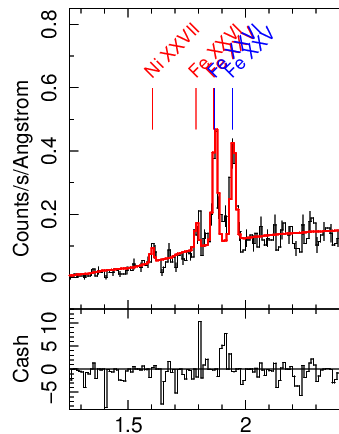
\includegraphics[width=\linewidth]{Chapters/Figures/short_pheno_part.png}
        \caption{1.25 - 2.4 \AA\ range of the Chandra HEG spectrum from the 20 ksec observation }
        \label{shortportion}
    \end{subfigure}%
    \hspace*{4em}
    \begin{subfigure}[t]{.3\textwidth}
        \centering
        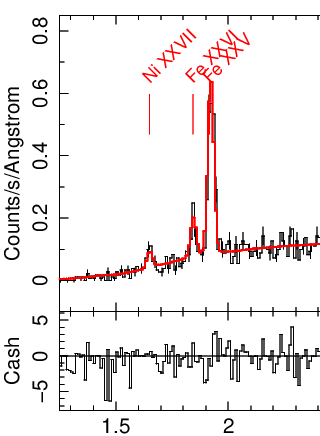
\includegraphics[width=\linewidth]{Chapters/Figures/long0_pheno_part.png}
        \caption{1.25 - 2.4 \AA\ range of the Chandra HEG spectrum from the first part of 96 ksec observation}
        \label{longportion}
    \end{subfigure}
    \label{portion}
\end{figure}


\begin{figure}[h!]
    \centering
    \begin{subfigure}[t]{.3\textwidth}
        \centering
        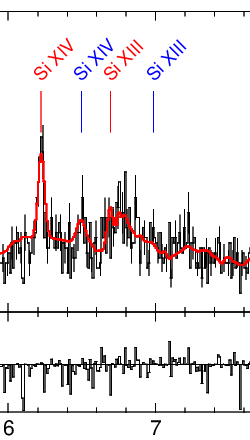
\includegraphics[width=\linewidth]{Chapters/Figures/short_pheno_part2.png}
        \caption{6-7.6 \AA\ range of the Chandra HEG spectrum from the 20 ksec observation }
        \label{shortportion2}
    \end{subfigure}%
    \hspace*{4em}
    \begin{subfigure}[t]{.3\textwidth}
        \centering
        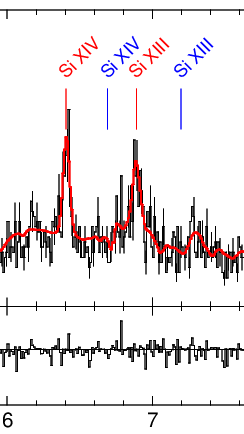
\includegraphics[width=\linewidth]{Chapters/Figures/long_pheno_part2.png}
        \caption{6-7.6 \AA\ range of the Chandra HEG spectrum from the first part of 96 ksec observation}
        \label{longportion2}
    \end{subfigure}
    \label{portion}
\end{figure}

\newpage
Applying the similar blind fitting method as the short observation, the line diagnostics for the long observation are shown in Table~\ref{tab:longlinefluxes_west} - \ref{tab:longlinefluxes_east}. With this model, Fe {\sc xxv} from the Western jet and Fe {\sc xxvi} from the Eastern jet could be fit with two Voigt profiles and thus line flux for each emission line was estimated.








\begin{deluxetable}{rccccr}
\tablecolumns{5}
\tablewidth{0pc}
\tabletypesize{\scriptsize}
\tablecaption{SS 433 Western Jet Line Diagnostics Using Voigt profiles for the 96 ksec Observation
\label{tab:longlinefluxes_west} }
\tablehead{\colhead{Identification}& \colhead{$\lambda_{\rm rest}$} & \colhead{$\lambda_{\rm obs}$} & \colhead{$z$}
    & \colhead{Flux}  & \colhead{$\sigma$}\\
  \colhead{} & \colhead{(\AA)} & \colhead{(\AA)} & \colhead{}
    & \colhead{($10^{-6}$ ph cm$^{-2}$ s$^{-1}$)} & \colhead{\AA}}
\startdata
Ni {\sc xxvii}&	1.592&	1.653$\pm$0.0032&	0.038$\pm$0.002&	257.6$\pm$54.6&	0.0108\\
		& &1.647$\pm$0.0023&	0.035$\pm$0.0014&	262.1$\pm$51.3&	0.0122\\
		& &1.649$\pm$0.002&	0.036$\pm$0.0013&	274.4$\pm$53.5&	0.012\\
		& &1.655$\pm$0.0017&	0.04$\pm$0.0011&	238.1$\pm$50.1&	0.0111\\
		& &1.644$\pm$0.0026&	0.033$\pm$0.0016&	149.3$\pm$48.4&	0.0121\\
					
					
Fe {\sc xxvi} &	1.78&	1.846$\pm$0.0013&	0.037$\pm$0.0007&	269.5$\pm$38.1&	0.0126\\
		& &1.845$\pm$0.0017&	0.037$\pm$0.001&	223.6$\pm$35.8&	0.0142\\
		& &1.842$\pm$0.0013&	0.035$\pm$0.0007&	290.9$\pm$37.7&	0.014\\
		& &1.847$\pm$0.0023&	0.037$\pm$0.0013&	209$\pm$33.6&	0.0129\\
		& &1.843$\pm$0.0015&	0.035$\pm$0.0008&	311.4$\pm$39.5&	0.0141\\
					
					
Fe {\sc xxv}&	1.855&	1.925$\pm$0.0012&	0.037$\pm$0.0006&	992.4$\pm$55.5&	0.0126\\
		& &1.92$\pm$0.0001&	0.035$\pm$0.0001&	807.8$\pm$49&	0.0142\\
		& &1.92$\pm$0.0001&	0.035$\pm$0.0001&	694.3$\pm$45.6&	0.014\\
		& &1.922$\pm$0.0008&	0.036$\pm$0.0004&	851.2$\pm$49.6&	0.0129\\
		& &1.92$\pm$0.0011&	0.035$\pm$0.0006&	787.4$\pm$50&	0.0141\\[1ex]
					
					
S {\sc xvi}&	4.73&	4.898$\pm$0.0017&	0.036$\pm$0.0004&	169.4$\pm$18.2&	0.0174\\
		& & 4.901$\pm$0.0026&	0.036$\pm$0.0005&	141.9$\pm$19&	0.0177\\
		& & 4.896$\pm$0.0029&	0.035$\pm$0.0006&	163.1$\pm$20.1&	0.0131\\
		& & 4.902$\pm$0.003&	0.036$\pm$0.0006&	152.4$\pm$21.3&	0.0161\\
		& & 4.89$\pm$0.0042&	0.034$\pm$0.0009&	203$\pm$24.4&	0.0211\\[1ex]
					
					
S {\sc xv}&	5.055&	5.222$\pm$0.0008&	0.033$\pm$0.0002&	78.8$\pm$16.9&	0.0186\\
		& &5.222$\pm$0.0012&	0.033$\pm$0.0002&	72$\pm$17.3&	0.0189\\
		& &5.222$\pm$0.002&	0.033$\pm$0.0004&	140.4$\pm$20.7&	0.014\\
		& &5.218$\pm$0.0047&	0.032$\pm$0.0009&	103.4$\pm$18.2&	0.0172\\
		& &5.213$\pm$0.0055&	0.031$\pm$0.0011&	202.4$\pm$23.6&	0.0225\\[1ex]
					
					
					
					
Si {\sc xiv}&	6.182&	6.405$\pm$0.0019&	0.036$\pm$0.0003&	215$\pm$13.9&	0.0227\\
		& &6.398$\pm$0.0019&	0.035$\pm$0.0003&	237.1$\pm$14&	0.0231\\
		& &6.399$\pm$0.0032&	0.035$\pm$0.0005&	251.2$\pm$23.4&	0.0172\\
		& &6.397$\pm$0.0015&	0.035$\pm$0.0002&	233.7$\pm$13.9&	0.021\\
		& &6.397$\pm$0.0025&	0.035$\pm$0.0004&	239.1$\pm$14.8&	0.0276\\[1ex]
					
					
					
					
Si {\sc xiii}r&	6.648&	6.859$\pm$0.0126&	0.032$\pm$0.0019&	20.1$\pm$1.8&	0.0244\\
		& &6.851$\pm$0.0152&	0.03$\pm$0.0023&	20$\pm$1.8&	0.0248\\
		& &6.859$\pm$0&	0.032$\pm$0&	20.1$\pm$15&	0.0184\\
		& &6.87$\pm$0.0058&	0.033$\pm$0.0009&	55.7$\pm$9.5&	0.0226\\
		& &6.909$\pm$0&	0.039$\pm$0&	39.1$\pm$11.3&	0.0296\\[1ex]
					
					
Si {\sc xiii}i&	6.687&	6.887$\pm$0.0032&	0.03$\pm$0.0005&	101.8$\pm$11.2&	0.0245\\
		& &6.889$\pm$0.0031&	0.03$\pm$0.0005&	115.6$\pm$10.9&	0.025\\
		& &6.89$\pm$0.0069&	0.03$\pm$0.001&	155.6$\pm$19.5&	0.0186\\
		& &6.93$\pm$0.0008&	0.036$\pm$0.0001&	75$\pm$0&	0.0227\\
		& &6.873$\pm$0.0026&	0.028$\pm$0.0004&	96.9$\pm$11.6&	0.0298\\[1ex]
					
					
Si {\sc xiii}f&	6.74&	6.916$\pm$0.0075&	0.026$\pm$0.0011&	50$\pm$0&	0.0247\\
		& &6.97$\pm$0&	0.034$\pm$0&	64.6$\pm$10.2&	0.0252\\
		& &6.97$\pm$0.0006&	0.034$\pm$0.0001&	152$\pm$15.5&	0.0187\\
		& &6.999$\pm$0.0077&	0.038$\pm$0.0011&	50$\pm$1.3&	0.0229\\
		& &6.991$\pm$0.0068&	0.037$\pm$0.001&	64.9$\pm$10.9&	0.03\\[1ex]
					
					
Mg {\sc xii}&	8.42&	8.708$\pm$0.0078&	0.034$\pm$0.0039&	103.6$\pm$13.7&	0.0309\\
		& &8.712$\pm$0.008&	0.035$\pm$0.004&	122.8$\pm$14.8&	0.0314\\
		& &8.712$\pm$0.0066&	0.035$\pm$0.004&	69.9$\pm$11.4&	0.0234\\
		& &8.709$\pm$0.0073&	0.034$\pm$0.0039&	66.6$\pm$11.5&	0.0286\\
		& &8.704$\pm$0.0065&	0.034$\pm$0.0039&	74.2$\pm$11.7&	0.0375\\

					
					
					
					

			
					





\enddata
\end{deluxetable}



\begin{deluxetable}{rcccr}
\tablecolumns{5}
\tablewidth{0pc}
\tabletypesize{\small}
\tablecaption{SS 433 Eastern Jet Lines Diagnostics Using Voigt profiles for the 96 ksec Observation
\label{tab:longlinefluxes_east} }
\tablehead{\colhead{Identification}& \colhead{$\lambda_{\rm rest}$} & \colhead{$\lambda_{\rm obs}$} & \colhead{$\Delta z$}
    & \colhead{Flux}  & \colhead{$\sigma$}&
  \colhead{} & \colhead{(\AA)} & \colhead{(\AA)} & \colhead{}
    & \colhead{($10^{-6}$ ph cm$^{-2}$ s$^{-1}$)} & \colhead{\AA}}
\startdata
S {\sc xvi}&	4.73&	5.14$\pm$0.0046&	0.0870$\pm$0.001&	32.6$\pm$11.2&	0.0174\\
		& &5.052$\pm$0.0086&	0.068$\pm$0.0018&	28.5$\pm$9.2&	0.0177\\
		& &5.06$\pm$0.0132&	0.070$\pm$0.0028&	25$\pm$6.2&	0.0131\\
		& &5.03$\pm$0.0076&	0.063$\pm$0.0016&	25$\pm$3.9&	0.0161\\
		& &5.037$\pm$0.0168&	0.065$\pm$0.0036&	53$\pm$19.4&	0.0211\\[1ex]
					
					
S {\sc xv}&	5.055&	5.404$\pm$0.014&	0.069$\pm$0.0028&	17.1$\pm$9.6&	0.0186\\
		&&5.409$\pm$0.0089&	0.07$\pm$0.0018&	33.7$\pm$16&	0.0189\\
		&&5.42$\pm$0.015&	0.072$\pm$0.003&	16.2$\pm$1.6&	0.014\\
		&&5.386$\pm$0.0078&	0.065$\pm$0.0015&	64.3$\pm$16.9&	0.0172\\
		&&5.401$\pm$0.0197&	0.069$\pm$0.0039&	24.3$\pm$16.3&	0.0225\\[1ex]
					
Si {\sc xiv}&	6.182&	6.687$\pm$0.0085&	0.082$\pm$0.0014&	60.1$\pm$10.5&	0.044\\
		&&6.69$\pm$0.0046&	0.082$\pm$0.0007&	67.3$\pm$11.2&	0.0494\\
		&&6.677$\pm$0.0059&	0.08$\pm$0.001&	126.5$\pm$20.2&	0.0487\\
		&&6.698$\pm$0.0051&	0.083$\pm$0.0008&	67$\pm$10.6&	0.0451\\
		&&6.685$\pm$0.0084&	0.081$\pm$0.0014&	74.3$\pm$11.6&	0.0493\\[1ex]
					
					
Si {\sc xiii}f&	6.74&	7.281$\pm$0&	0.08$\pm$0&	26.7$\pm$9.5&	0.0479\\
		&&7.331$\pm$0&	0.088$\pm$0&	37.4$\pm$9.7&	0.0538\\
		&&7.347$\pm$0.0113&	0.09$\pm$0.0017&	217.1$\pm$17.3&	0.0531\\
		&&7.333$\pm$0.0077&	0.088$\pm$0.0011&	37.6$\pm$9.6&	0.0491\\
		&&7.331$\pm$0&	0.088$\pm$0&	61.9$\pm$11.2&	0.0537\\




\enddata
\end{deluxetable}


















